
\chapter{A novel data encoding technique}

The paper \cite{P_rez_Salinas_2020} is a groundbreaking paper in quantum machine learning.\\
Significant effort by the quantum machine learning community has been dedicated to deepening our understanding of 
quantum re-uploading models, leading to a growing body of literature investigating them.\\
As we studied this paper, some natural questions emerged and we decided to investigate them by designing
a novel data encoding technique for quantum re-uploading models, whose main goal is to classify 
\textit{high-dimensional} and \textit{structured} datasets\footnote[1]{The term \textit{structured} is 
used to indicate that the components of each datapoint in the dataset may be highly correlated.}.\\
In the following sections we will discuss the questions emerged from reading the original data re-uploading
paper and a new quantum machine learning algorithm.

\section{Questions on data re-uploading}

The groundbreaking paper on the data re-uploading technique \cite{P_rez_Salinas_2020} does not address some crucial 
question, which could be an interesting starting point for future research:

\begin{itemize}
    \item\label{question:first} Is this encoding technique effective when dealing with high-dimensional datasets?\\
    The investigation conducted by Salinas et al focused on 2D, 3D and 4D data, hence this raises the natural
    question if this encoding method can deal with datasets of higher dimension.
    \item\label{question:second} Is this encoding technique effective when dealing with structured dataset (as images)?\\
    The original paper tested the data re-uploading encoding method to distinguish if a certain point was 
    inside or outside a certain geometrical boundary (circle, sphere, annulus, ...).
    However it did not investigate its performance on datasets, whose each datapoint's components could 
    be correlated to each other.
    Therefore, this raises another natural question which is if the data re-uplaoding technique can handle datasets
    like images, whose pixels are highly correlated to the sorrounding pixels.
\end{itemize}

We tried to answer to these questions by designing a new quantum machine learning algorithm based on the
data re-uploading technique.\\
I will discuss this new algorithm in the following section.

\section{Block re-uploading}

This new algorithm, which we call \textit{block re-uploading}, is inspired by classical convolutional neural 
networks and its main goal is to classify images.
Images are composed of pixels, and each pixel is typically represented as a vector of three 
values corresponding to the intensity of the primary colors: red, green, and blue (RGB). 
Each of these values typically ranges from 0 to 255 in an 8-bit color depth image, which is common in 
digital images.\\
It is essential to observe that not all the information contained in an image is essential for
classification purposes.
Indeed, many preprocessing techniques, such as PCA, have been used in the literature to reduce 
the amount of information fed into a (quantum) neural network.\\
to preserve information redundancy in the images and maintain the full dimensionality of the dataset. 
This approach aligns with our objective of addressing question \ref{question:first}.\\

The fundamental idea behind the \textit{block re-uploading} algorithm is based on the observation that 
neighboring pixels in an image are highly correlated. 
Consequently, we chose to divide each image into blocks and upload each block onto a separate qubit\footnote[1]{We wanted to make these blocks as similar to each other as possible, but dimensional constraints 
prevented them from being identical. For instance, an $8\times8$ image cannot be divided in three
identical blocks.} (figure \ref{fig:block}).\\

\begin{figure}[h]
    \centering
    \begin{subfigure}[b]{0.45\textwidth}
        \centering
        \includegraphics[scale=0.65]{sections/chapters/Chapter6/Images/Blocks-Circuit/blocks.pdf}
    \end{subfigure}
    \begin{subfigure}[b]{0.45\textwidth}
        \centering
        \includegraphics[scale=0.75]{sections/chapters/Chapter6/Images/Blocks-Circuit/circuit.pdf}
    \end{subfigure}
    \caption{An image with even width and height can be divided into exactly four equal blocks. 
    Each block will then be encoded onto a separate qubit. As we will explain in the next paragraph the 
    \textit{block re-uploading} architecture has three components per layer: embedding circuit, 
    entanglement circuit, pooling circuit.}
    \label{fig:block}
\end{figure}

Apart from answering to the questions \ref{question:first}, \ref{question:second}, our main goal was to 
investigate the \textit{Depth vs Width trade-off}.
The \textit{Depth vs Width trade-off} can be more explicitly referred to as the
\textit{Sequential vs Parallel uploading trade-off}.
If we do not split the image into blocks, the entire image will be encoded into a single qubit, 
resulting in sequential distribution of information across the quantum circuit. 
In contrast, if we divide the image into blocks and encode each block onto a separate qubit, 
the information will be distributed both sequentially and in parallel. As the number of blocks increases, 
the distribution of information becomes progressively more parallel, reaching the limit where each 
block consists of a single pixel.
This trade-off raises the natural questions: \textit{which distribution is better? Sequential or parallel?}.
As is common when evaluating trade-offs, the optimal solution often lies between the two extremes. 
Therefore, we predict that the best approach to distributing information across the quantum circuit 
will involve a balanced mix of sequential and parallel encoding.\\

\begin{figure}
    \centering
    \begin{subfigure}[b]{0.3\textwidth}
        \centering
        \includegraphics[width=\textwidth]{sections/chapters/Chapter6/Images/Sequential-Parallel/sequential_blocks.pdf}
        \label{fig:sequential-block}
    \end{subfigure}
    \hfill
    \begin{subfigure}[b]{0.3\textwidth}
        \centering
        \includegraphics[width=\textwidth]{sections/chapters/Chapter6/Images/Sequential-Parallel/proportionate_blocks.pdf}
        \label{fig:prop-block}
    \end{subfigure}
    \hfill
    \begin{subfigure}[b]{0.3\textwidth}
        \centering
        \includegraphics[width=\textwidth]{sections/chapters/Chapter6/Images/Sequential-Parallel/parallel_blocks.pdf}
        \label{fig:parallel-block}
    \end{subfigure}
    \hfill
    \begin{subfigure}[b]{0.3\textwidth}
        \centering
        \includegraphics[width=\textwidth]{sections/chapters/Chapter6/Images/Sequential-Parallel/sequential.pdf}
        \label{fig:sequential-circ}
    \end{subfigure}
    \hfill
    \begin{subfigure}[b]{0.3\textwidth}
        \centering
        \includegraphics[width=\textwidth]{sections/chapters/Chapter6/Images/Sequential-Parallel/proportionate.pdf}
        \label{fig:prop-circ}
    \end{subfigure}
    \hfill
    \begin{subfigure}[b]{0.3\textwidth}
        \centering
        \includegraphics[width=\textwidth]{sections/chapters/Chapter6/Images/Sequential-Parallel/parallel.pdf}
        \label{fig:parallel-circ}
    \end{subfigure}
    \caption{This figure shows three possible splitting of a $4\times4$ image and the corresponding 
    circuit. 
    If the image is not divided into blocks, it will be uploaded to a single qubit, 
    representing a fully-sequential approach. 
    Dividing the image into 4 blocks results in a 4-qubit architecture, 
    positioning it roughly at the midpoint of the sequential-parallel spectrum.
    If the image is divided into 16 blocks, each block will contain only 1 pixel. 
    This scenario exemplifies the fully-parallel uploading limit, as each pixel is assigned to 
    a separate qubit.}
    \label{fig:three-splitting}
\end{figure}



The \textit{block re-uploading} algorithm is a layered algorithm and each layer has three components: 
an embedding circuit, an entanglement structure and a pooling circuit.

\begin{figure}[h]
    \centering
    \includegraphics[scale=0.65]{sections/chapters/Chapter6/Images/Two-Layers-A/two_layer.pdf}
    \caption{A four qubits and two layers \textit{block re-uploading} architecture. Each layer has three 
    components: an embedding circuit, an entanglement structure and a pooling circuit.
    Layers are separated by another entanglement structure.}
\end{figure}

\paragraph{Embedding}
The embedding component is responsible to encode each block of an image onto a different qubit of 
the quantum circuit (figure \label{fig:block}).\\
For instance, an $8\times8$ image can be divided in 4 identical $4\times4$ blocks. 
Therefore, each $4\times4$ block is a 16 dimensional vector which requires 
$\left\lceil \frac{d}{3} \right\rceil = \left\lceil \frac{16}{3} \right\rceil = 6$ unitary matrices 
to be encoded onto a qubit.
In particular, each block needs 16 rotation gates, one per pixel.
Therefore, the unitary matrices necessary to encode a block $\bm{x} = (x_1, x_2, ..., x_{16})$ will be:

\begin{align}
    U^1_1(\bm{\phi_1}) &= U_1(\bm{x}, \bm{\theta_1}) = R_Z(\phi_{1,1}) R_Y(\phi_{1,2}) R_Z(\phi_{1,3}) \\
    U^1_2(\bm{\phi_2}) &= U_2(\bm{x}, \bm{\theta_2}) = R_Z(\phi_{2,1}) R_Y(\phi_{2,2}) R_Z(\phi_{2,3}) \\
    &\vdots \\
    U^1_6(\bm{\phi_6}) &= U_1(\bm{x}, \bm{\theta_6}) = R_Z(\phi_{6,1}) R_Y(\phi_{6,2}) R_Z(\phi_{6,3}) 
\end{align}

where $\bm{\theta_i} = (w_{i,1}, w_{i,2}, w_{i,3}, b_{i,1})$.
The angles will be defined as a linear combination of pixels and weights, for example $\bm{\phi_1}$:

\begin{align}
    \phi_{1,1} &= x_1 \cdot w_{1,1} + b_{1,1} \\
    \phi_{1,2} &= x_2 \cdot w_{1,2} + b_{1,2} \\
    \phi_{1,3} &= x_3 \cdot w_{1,3} + b_{1,3} \\
\end{align}


\begin{figure}[h]
    \centering
    \begin{quantikz}
        &&& \gate{U^1_1} & \gate{U^1_2} & \gate{U^1_3} & \gate{U^1_4} & \gate{U^1_5} & \gate{U^1_6} &&& \\
        &&& \gate{U^2_1} & \gate{U^2_2} & \gate{U^2_3} & \gate{U^2_4} & \gate{U^2_5} & \gate{U^2_6} &&& \\
        &&& \gate{U^3_1} & \gate{U^3_2} & \gate{U^3_3} & \gate{U^3_4} & \gate{U^3_5} & \gate{U^3_6} &&& \\
        &&& \gate{U^4_1} & \gate{U^4_2} & \gate{U^4_3} & \gate{U^4_4} & \gate{U^4_5} & \gate{U^4_6} &&& \\
    \end{quantikz}
    \caption{Embedding circuit for an $8\times8$ image divided in 4 identical $4\times4$ blocks.}
\end{figure}


\paragraph{Entanglement structure}
Since each block is correlated with its neighboring blocks, we decided to use an entanglement 
structure in which entangling gates create connections between adjacent blocks.
We chose CZ, as the only entangling gate.
Therefore, the entanglement structure aims to ensure that each qubit shares information only with 
qubits that contain related information.

\begin{figure}[h]
    \centering
    \begin{quantikz}
        &&& \ctrl{1} & \ctrl{2}   &       &     &&&&\\
        &&& \targ{}  &    &       &   \ctrl{2}    &     &&&\\
        &&&    &        \targ{}    &       &   & \ctrl{1}   &&&\\
        &&&    &     &    &       \targ{}   &   \targ{}  &&&\\
    \end{quantikz}
    \caption{Entanglement structure for an image divided in 4 blocks. The first qubit will 
    communicate with the second one and the third one, as the first block is adjacent to the second and the third one.
    Then, the second block will be connected to the fourth one and the third to fourth one.}
\end{figure}

\paragraph{Pooling}
In classical machine learning the pooling layers are used to make the network less sensitive to small translations 
and distortions in the input data.\\
Therefore, we decided to mimic the pooling component of classical convolutional neural networks, by 
adding an X rotation gate per qubit, whose angle is defined as the linear combination of the max (or average) value 
of a block and weights.
Therefore, if we consider again an $8\times8$ image divided in 4 identical $4\times4$ blocks: 

\begin{align}
    \bm{x_1} &= (x_{1,1}, x_{1,2}, ..., x_{1,16}) 
    \qquad
    \rightarrow
    \qquad
    max(\bm{x_1}) \\
    \bm{x_2} &= (x_{2,1}, x_{2,2}, ..., x_{2,16}) 
    \qquad
    \rightarrow
    \qquad
    max(\bm{x_2}) \\
    \bm{x_3} &= (x_{3,1}, x_{3,2}, ..., x_{3,16}) 
    \qquad
    \rightarrow
    \qquad
    max(\bm{x_3}) \\
    \bm{x_4} &= (x_{4,1}, x_{4,2}, ..., x_{4,16}) 
    \qquad
    \rightarrow
    \qquad
    max(\bm{x_4}) \\
\end{align}

the angles of the four X rotation gates will be:

\begin{align}
    \phi_{1} &= max(\bm{x_1}) \cdot w_{1} + b_{1} \\
    \phi_{2} &= max(\bm{x_2}) \cdot w_{2} + b_{2} \\
    \phi_{3} &= max(\bm{x_3}) \cdot w_{3} + b_{3} \\
    \phi_{4} &= max(\bm{x_4}) \cdot w_{4} + b_{4} \\
\end{align}


\begin{figure}[h]
    \centering
    \begin{quantikz}
        &&& \gate{R^1_x} &&& \\
        &&& \gate{R^2_x} &&& \\
        &&& \gate{R^3_x} &&& \\
        &&& \gate{R^4_x} &&& \\
    \end{quantikz}
    \caption{Pooling circuit for a 4 qubit architecture.}
\end{figure}


Moreover, another fundamental concept of the \textit{block re-uploading} algorithm is that the 
number of qubits of the architecture corresponds to the number of blocks in which we divided the 
image, our main goal is to understand what is the optimal archi


\section{Numerical results}

We conducted several numerical test on the \textit{block re-uploading} architecture:

\begin{itemize}
    \item Classification.\\
    We conducted both binary and multi-class classification.
    \item Dataset.\\
    We used both the MNIST digit and MNIST fashion datasets, which are both grayscale $28\times28$ pixels images.
    \item Image size.\\
    We used different down-scaling of the MNIST dataset:
    $4\times4$, $8\times8$, $12\times12$, $14\times14$, $16\times16$, $18\times18$.
    \item Decoding observable.\\
    Every quantum machine learning algorithm has a \textit{decoding} component at the end of it, which consists in 
    measuring an observable to extract information from the PQC.
    The observable that we chose are: \textit{global Pauli Z}, which is the tensor product of n (number of qubits
    of the circuit) Pauli Z, \textit{local Pauli Z}, which is only one Pauli Z.
    Regarding the local Pauli Z measurement, in the block re-uploading architecture with multiple qubits, 
    we had the option to measure any qubit. However, we consistently chose to measure only the first qubit.
    \item Architectures.\\
    We studied three different architectures.
    The first one has only the embedding component, the second one has both the embedding and pooling components, the third
    one has the embedding, entanglement and pooling components.
    These architectures differ in terms of the number of gates and parameters they utilize, as shown by
    figure  
\end{itemize}

\begin{figure}[h]
    \centering
    \includegraphics[scale=0.7]{sections/chapters/Chapter6/Images/Architectures/embedding.pdf}
    \caption{This is the baseline model. This model only re-uploads multiple times the data in the circuit.}
    \label{arc:embed}
\end{figure}

\begin{figure}[h]
    \centering
    \includegraphics[scale=0.7]{sections/chapters/Chapter6/Images/Architectures/embedding_pooling.pdf}
    \caption{This model has both the embedding and the pooling circuit.}
    \label{arc:embed-pooling}
\end{figure}

It is essential to keep in mind that by increasing the size of images the number of embedding gates will
increase, hence an embedding architecture (baseline model) for $4\times4$ images will be different 
from the embedding architecture for $8\times8$.
The comparison between the baseline model for different sizes of the images is shown in figure 
\ref{arc:embed-pooling}

\begin{figure}[h]
    \centering
    \includegraphics[scale=0.4]{sections/chapters/Chapter6/Images/Image-Size/Heatmap-Comparison-Arch.pdf}
    \caption{The first row displays the number of parametric gates (excluding entangling gates) for 
    different image sizes across two architectures: embedding and embedding + pooling.
    The second row displays the number of trainable parameters for 
    different image sizes across two architectures: embedding and embedding + pooling.}
    \label{arc:embed-pooling}
\end{figure}


The following sections will discuss the \textit{generalization} capabilities and the 
\textit{trainability} of the \textit{block re-uploading} architecture.
I will group all the architectures combination in three main categories: \textit{narrow-deep} 
(few qubits and numerous layers), \textit{wide-shallow} (many qubits and few layers), \textit{proportionate}
(every other architecture). 


\subsection{Local 4x4}


\subsection{Global 4x4}


\subsection{Local 8x8}

\begin{figure}[h]
    \centering
    \includegraphics[scale=0.35]{sections/chapters/Chapter6/Images/Heatmaps/Local-Heatmaps/Heatmap-Both-8x8-L.pdf}
    \caption{This heatmap shows the training and validation accuracy for architectures with 1-15 qubits and
    1-6 layers for the $8\times8$ down-scaled MNIST digits and fashion dataset using a global Pauli Z.}
    \label{fig:heatmap-8x8-L}
\end{figure}
By looking at figure \ref{fig:heatmap-8x8-L}, we can distinguish 
three different behaviours:

\begin{enumerate}
    \item \textbf{Deep-Narrow}.\\
    As the number of layers increases in narrow architectures (1, 2, or 3 qubits), their capacity to 
    generalize diminishes, leading to overfitting. This occurs because the increase in layers corresponds 
    to a rise in the number of trainable parameters (see figure \ref{arc:embed-pooling}).\\
    As a result, the architecture becomes overparameterized, allowing it to capture even minor 
    fluctuations in the training dataset, which reduces its ability to generalize effectively to new, 
    unseen data.
    \item \textbf{Shallow-Wide}.\\
    As the number of qubits (width) increases both training and validation accuracy of 
    single-layer architectures (shallow) drop drastically.
    As the width of the architecture increases, a greater degree of entanglement is required to 
    effectively distribute information across all qubits. However, shallow architectures lack 
    sufficient entangling gates to achieve this, resulting in an inability to fully capture and 
    “understand" the complete picture.\\
    However, by comparing training and validation accuracy, although both decrease as 
    the width increases, there is no evidence of overfitting.\\
    We can conclude that, as the architecture widens, entanglement becomes increasingly crucial for the 
    architecture to effectively ”understand” the image.
    \item \textbf{Proportionate}.\\
    In proportionate architectures (those that are neither shallow-wide nor deep-narrow) overfitting 
    tends to diminish. As the number of layers and qubits increases, the \textit{block re-uploading} 
    introduces a richer set of entanglement structures, enabling more effective information sharing 
    across all qubits. This reduction in overfitting as entanglement grows raises some natural questions:
    \textit{Could entanglement be a factor that resists overfitting?}, 
    \textit{Might entanglement serve as a source of regularization?}.
\end{enumerate}


\subsection{Global 8x8}

\begin{figure}[h]
    \centering
    \includegraphics[scale=0.35]{sections/chapters/Chapter6/Images/Heatmaps/Global-Heatmaps/Heatmap-Both-8x8-G.pdf}
    \caption{This heatmap shows the training and validation accuracy for architectures with 1-15 qubits and
    1-6 layers for the $8\times8$ down-scaled MNIST digits and fashion dataset using a global Pauli Z.}
    \label{fig:heatmap-8x8-G}
\end{figure}


By looking at figure \ref{fig:heatmap-8x8-G}, we can notice 
several interesting behaviours:

\begin{itemize}
    \item \textbf{Deep vs Shallow}: Global vs Local.\\
    Shallow architectures clearly outperform deep ones, with overfitting becoming more pronounced 
    as the number of layers (depth) increases.\\
    This behavior is particularly noteworthy and contrasts with the numerical results observed 
    using a local Pauli Z.
    \item \textbf{Deep-Narrow}: Global vs Local.\\
    As stated in the previous point, overfitting is way more pronounced with respect to the local case.\\
    \item \textbf{Shallow-Wide}: Global vs Local.\\
    Shallow-Wide architectures (1-layer architectures) show an interesting behaviour: as the number of 
    qubits increases both training and validation accuracy of single-layer architectures 
    do not drop drastically, but remain stable.\\
    The lack of sufficient entanglement to share information across all qubits is compensated by 
    measuring a global observable, which effectively captures the dispersed information throughout the 
    circuit.
    \item \textbf{Proportionate}: Global vs Local.\\
    Proportionate architectures (center and bottom-right area of the heatmap) do not exhibit overfitting. \\
    However, they generally perform worse than their local counterparts.
 \end{itemize}

\subsection{Local 12x12}
\begin{figure}[h]
    \centering
    \includegraphics[scale=0.3]{sections/chapters/Chapter6/Images/Heatmaps/Local-Heatmaps/Heatmap-Both-12x12-L.pdf}
    \caption{This heatmap shows the training and validation accuracy for architectures 
    trained on the $12\times12$ down-scaled MNIST digits and fashion dataset using a local Pauli Z.}
    \label{fig:heatmap-12x12-L}
\end{figure}

By enlarging the images, we observe a consistent trend across all categories 
(deep-narrow, shallow-wide, proportionate): the training accuracy remains basically the same, whereas we 
can notice an increasing presence of overfitting.
We can observe that the general behaviour of the validation accuracy seen with $8\times8$ images is 
similarly observed with $12\times12$ images, but \textit{shifted to the left by one or two layers}\footnote[1]{We are comparing only the local case. 
By general behaviour we intend that as the architecture becomes deeper overfitting becomes more 
pronounced.}. This shift 
occurs because the increased number of parameters in each layer makes the model more prone to overfitting.\\

By looking at figure \ref{fig:heatmap-12x12-L}, we can distinguish 
three different behaviours:

\begin{itemize}
    \item \textbf{Deep-Narrow}: $8\times8$ vs $12\times12$.\\
    Overfitting is more pronounced for deep-narrow architectures.\\
    In both the $8\times8$ and $12\times12$ cases, overfitting worsens as the number of layers increases. \\
    Training accuracy remains stable for $8\times8$ images, but for $12\times12$ images, 
    it decreases with the addition of more layers.
    \item \textbf{Shallow-Wide}: $8\times8$ vs $12\times12$.\\
    In the $8\times8$ case we noticed the drastic drop for both the validation and training accuracy for 
    architectures wider than 8 qubits, so since for the $12\times12$ we did not train architectures wider than 
    8 qubits we cannot conclude that we would see the same drastic drop.
    However, since deep-narrow and proportionate architectures in the $12\times12$ case did not show 
    significant differences with the $8\times8$ case we can assume that even Shallow-Wide architectures will
    not show significant differences.\\
    The effect of distributing information across more qubits in shallow architectures is particularly 
    evident in the $12\times12$ case. For instance, when examining 2-layer architectures vertically, 
    it's clear that spreading the information across more qubits significantly enhances both training and 
    validation accuracy.
    \item \textbf{Proportionate}: $8\times8$ vs $12\times12$.\\
    Again overfitting tends to disappear. \\
 \end{itemize}

\subsection{Global 12x12}
\begin{figure}[h]
    \centering
    \includegraphics[scale=0.3]{sections/chapters/Chapter6/Images/Heatmaps/Global-Heatmaps/Heatmap-Both-12x12-G.pdf}
    \caption{This heatmap shows the training and validation accuracy for architectures with 1-15 qubits and
    1-6 layers for the $12\times12$ down-scaled MNIST digits and fashion dataset using a global Pauli Z.}
    \label{fig:heatmap-12x12-G}
\end{figure}

By looking at figure \ref{fig:heatmap-12x12-G}, we can distinguish 
three different behaviours:

\begin{itemize}
    \item \textbf{Deep-Narrow}: $8 \times 8$ vs $12 \times 12$.\\
    
    \item \textbf{Shallow-Wide}: $8 \times 8$ vs $12 \times 12$.\\
    
    \item \textbf{Proportionate}: $8 \times 8$ vs $12 \times 12$.\\
    
 \end{itemize}

\subsection{Local 14x14}
\begin{figure}[h]
    \centering
    \includegraphics[scale=0.3]{sections/chapters/Chapter6/Images/Heatmaps/Local-Heatmaps/Heatmap-Both-14x14-L.pdf}
    \caption{This heatmap shows the training and validation accuracy for architectures for the $14\times14$ down-scaled MNIST digits and fashion dataset using a local Pauli Z.}
    \label{fig:heatmap-14x14-L}
\end{figure}

By looking at figure \ref{fig:heatmap-14x14-L}, we can distinguish 
three different behaviours:

\subsection{Global 14x14}
\begin{figure}[h]
    \centering
    \includegraphics[scale=0.3]{sections/chapters/Chapter6/Images/Heatmaps/Global-Heatmaps/Heatmap-Digits-14x14-G.pdf}
    \caption{This heatmap shows the training and validation accuracy for the $14\times14$ 
    down-scaled MNIST digits dataset using a global Pauli Z.}
    \label{fig:heatmap-14x14-G}
\end{figure}


By enlarging the images to $14\times14$, we can again notice a \textit{shift to the left by 
one or two layers} of the validation accuracy with respect to the $12\times12$ local case (figure 
\ref{fig:heatmap-14x14-L}). Once again, this shift 
occurs because the increased number of parameters in each layer makes the model more prone to overfitting.
The training accuracy for the $14\times14$ is essentially the same for both the $8\times8$ and 
$12\times12$ cases.

The remarks regarding the \textit{Deep-Narrow}, \textit{Shallow-Wide}, and \textit{Proportionate} 
architectures are consistent with those made in Section \ref{sssec:local-12} for the $12\times12$ case.
By examining Figure \ref{fig:heatmap-14x14-L}, no new behavior is observed that hasn't already 
been discussed in the $8\times8$ and $12\times12$ comparisons.

\subsection{Local 16x16 and 18x18}
\begin{figure}[h]
    \centering
    \includegraphics[scale=0.3]{sections/chapters/Chapter6/Images/Heatmaps/Local-Heatmaps/Heatmap-Digits-16-18-L.pdf}
    \caption{This heatmap shows the training and validation accuracy for architectures for the $16\times16$ and $18\times18$ down-scaled MNIST digits
     dataset using a local Pauli Z.
     Some training sessions run for 150 epochs (e.g., $16 \times 16$: 2 qubits, $18 \times 18$: 
     1 qubit, 3 qubits), while others are extended to 200 epochs.}
    \label{fig:heatmap-14x14-L}
\end{figure}

By looking at figure \ref{fig:heatmap-14x14-L}, we can distinguish 
three different behaviours:

\subsection{Comparing few-qubits architectures}
\begin{figure}[h]
    \centering
    \includegraphics[scale=0.3]{sections/chapters/Chapter6/Images/Heatmaps/Local-Heatmaps/Heatmap-Digits-Small-Arch-L-train.pdf}
    \caption{}
    \label{fig:heatmap-Small-train}
\end{figure}

\begin{figure}[h]
    \centering
    \includegraphics[scale=0.3]{sections/chapters/Chapter6/Images/Heatmaps/Local-Heatmaps/Heatmap-Digits-Small-Arch-L-val.pdf}
    \caption{}
    \label{fig:heatmap-Small-val}
\end{figure}


\subsection{Comparing single-layer architectures}
\begin{figure}[h]
    \centering
    \includegraphics[scale=0.5]{sections/chapters/Chapter6/Images/Single-Layer/single-layer-comparison-compact-local-8x8.pdf}
    \caption{This figure shows the training and validation loss and accuracy for single-layer architectures
    trained on the $8\times8$ down-scaled MNIST digits dataset using a \textbf{local} Pauli Z.}
    \label{fig:Single-loss-local}
\end{figure}

\begin{figure}[h]
    \centering
    \includegraphics[scale=0.5]{sections/chapters/Chapter6/Images/Single-Layer/single-layer-comparison-compact-global-8x8.pdf}
    \caption{This figure shows the training and validation loss and accuracy for single-layer architectures
    trained on the $8\times8$ down-scaled MNIST digits dataset using a \textbf{global} Pauli Z.}
    \label{fig:Single-loss-global}
\end{figure}


As observed in subsection \ref{sssec:num1} and illustrated by the first column of the heatmap 
\ref{fig:heatmap-8x8-L}, there is a notable decrease in accuracy as the architectures become wider.\\
This behavior is not observed in the global case: as shown in heatmap \ref{fig:heatmap-8x8-G}, 
the accuracy remains stable as the architectures become wider, without the same significant drop.
This difference between the local and global cases can be attributed to the \textit{entanglement dynamics} and 
the \textit{type of observable used for decoding}. 
In the local case, the lack of entanglement limits information sharing across qubits. 
In contrast, a global observable, which aggregates information from all qubits, mitigates the 
impact of limited information sharing in wider architectures.\\

This intriguing behavior warrants a detailed discussion. 
In this section, we will analyze the evolution of loss functions and accuracies over 200 epochs, 
as illustrated in figures \ref{fig:Single-loss-local} and \ref{fig:Single-loss-global}.

\begin{itemize}
    \item \textbf{Training Loss}.\\ 
    An examination of the global and local training losses reveals that the 1-qubit configuration 
    has the lowest loss, with losses increasing as the number of qubits 
    increases\footnote[1]{This observation holds true except for the global 11-qubit configuration, 
    which appears as an outlier. This anomaly could be addressed by conducting a statistical analysis 
    with multiple training runs using different initialization seeds.}.
    As the number of qubits increases, the architecture becomes more challenging to train, resulting 
    in a higher loss function plateau in performance.
    \item \textbf{Validation Loss}.\\ 
    For validation loss, the trend of loss decreasing with the number of qubits is consistent 
    in the local case but not in the global case, where the losses are mixed.
    \item \textbf{Training-Validation Accuracy}.\\
    The local accuracy exhibits numerical instability as the number of qubits increases. 
    Initially smooth, the accuracy becomes increasingly "stair-stepped" with more qubits, 
    and eventually levels off, becoming constant for 14-qubit and 15-qubit architectures. 
    This progression illustrates how numerical instability becomes more pronounced with a 
    larger number of qubits.\\
    We can assert that the local 9-qubits (or 8-qubits) architecture represents the threshold beyond which numerical 
    instability becomes more pronounced.\\
    It is noteworthy that \textit{numerical instability is not observed in the global case}. 
    A possible explanation is that a global observable aggregates more information, which may 
    help mitigate the numerical instability seen when measuring an individual qubit.
\end{itemize}









\subsection{Conclusions}

\subsection{Outlook}

\begin{comment}
\section{Data Re-Uploading}

\cite{P_rez_Salinas_2020} introduced the \textit{re-uploading} encoding technique,
drawing inspiration from classical neural networks.
The key idea that inspired Salinas et al is that a feed-forward neural network processes data several times
(in each layer), one for each neuron in the considered hidden layer. 
Therefore, strictly speaking, data is \textit{re-uploaded} multiple times onto the neural network.
This key concept is illustrated in figure~\ref{Fig:schemes}.


% \subcaption[⟨list entry⟩]{⟨heading⟩}[⟨width⟩][⟨inner-pos⟩]{⟨contents⟩}
% list entry: nome interno che verrà usato se generata la lista delle figure.
% heading: subcaption
% width: larghezza del parbox creato
% inner-pos: posizione che avrà l'immagine nel parbox
% contents: immagine
\begin{figure}
    \centering
    \subcaptionbox[A]{Neural Network}[.4\textwidth][c]{
        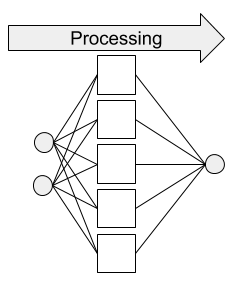
\includegraphics[width=0.25\textwidth]{sections/chapters/Chapter6/Images/Neural_network.png}
        }
    \subcaptionbox[B]{Quantum circuit with re-uploading}[.4\textwidth][c]{
        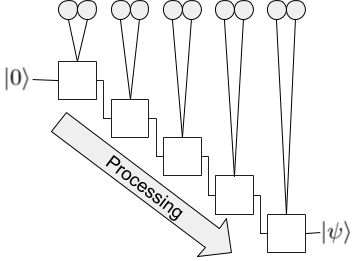
\includegraphics[width=0.5\textwidth]{sections/chapters/Chapter6/Images/Quantum_scheme.png}
        }
    \caption{
        Schemes of a one layer neural network and a single-qubit quantum circuit with data re-uploading.
        In the neural network the data is uploaded in each neuron of the hidden layer, hence data is 
        \textit{re-uploaded} multiple times.
        In a similar way the data is introduced classically numerous times in the circuit.
        The key difference between the two architectures is that each neuron of a neural network processes the 
        data in parallel and simultaneously, whereas the single-qubit quantum circuit with data re-uploading 
        processes the data sequentially.}
\label{Fig:schemes}
\end{figure}

In a single-qubit quantum circuit with data re-uploading, data is introduced as a rotation of the qubit.
Since every unitary can be expressed as the product of three rotation gates, we can define the angles as a linear
combination of weights and coordinates of the data\footnote[1]{Just like in a neuron of neural network.}.

\begin{equation}
    U(\bm{\phi}) = R_Z(\phi_1) R_Y(\phi_2) R_Z(\phi_3)
\label{}
\end{equation}

For instance, if data is 3-dimensional $\bm{x} = (x_1, x_2, x_3)$:

\begin{align}
    \phi_1 &= x_1 \cdot w_1 + b_1 \\
    \phi_2 &= x_2 \cdot w_2 + b_2 \\
    \phi_3 &= x_3 \cdot w_3 + b_3 \\
\end{align}

If data has a dimension greater than 3, we will need more than one unitary to encode a datapoint.
In general, if data has dimension \textit{d} we will need \(\left\lfloor \frac{d}{3} \right\rceil\) unitaries.
Each repetition of this \(\left\lfloor \frac{d}{3} \right\rceil\) unitaries to encode the data constitutes 
one layer of the architectures.

\begin{figure}
    \centering
    \begin{quantikz}
        \lstick{$\ket{0}$} &&& \gate{U(\phi_1, x)} 
        \gategroup[1,steps=1, style={dashed,rounded corners,fill=blue!20,inner xsep=6pt}, background, label style={label
        position=below, yshift=-0.4cm}]{L(1)} 
        &&& \ \ldots \ &&& \gate{U(\phi_N, x)} 
        \gategroup[1,steps=1, style={dashed,rounded corners,fill=blue!20,inner xsep=6pt}, background, label style={label
        position=below, yshift=-0.4cm}]{L(N)}
        &&& \meter{}
    \end{quantikz}
    \caption{The quantum circuit is divided into layers L(i), which constitutes the building blocks of this 
    architecture.}
\end{figure}

\end{comment}


